\section{Ecuación de Renderizado}
La ecuación de renderizado fue introducida por Kajiya  en 1986 \cite{kajiya86}. Esta ecuacion describe en cada punto $x$ de una superficie y en cada dirección $\Theta$, la radiancia saliente $L(x\to\Theta)$ en ese punto y esa dirección.

El objetivo de un algoritmo para el cálculo de iluminación global es aproximar el resultado de esta ecuación. En esta ecuación asumimos que no existen medios participantes como objetos translúcidos como ya fue explicado en la sección \ref{sec:surface_rep}. También asumimos que la luz se propaga de forma inmediata por tanto la distribución de la luz, ya en un estado estacionario, se obtiene inmediatamente. 

\subsection{Formulación Hemisférica}
La formulación hemisférica de la ecuación de renderizado es una de las más utilizadas \cite{advanced_gi2006}. Esta formulación se obtiene utilizando la propiedad de conservación de energía en el punto $x$. Asumiendo que $L_{e}(x\to\Theta)$ representa la radiancia emitida por la superficie en el punto $x$ con dirección saliente $\Theta$ y $L_{r}(x\to\Theta)$ representa la radiancia reflectada por la superficie en el punto $x$ en dirección $\Theta$.

Por conservación de energía, el total de la radiancia saliente en un punto y dirección particular es la suma de la radiancia emitida y la radiancia reflectada en este punto de la superficie y dirección. La radiancia saliente $L(x\to\Theta)$ es expresada en términos de $L_{e}(x\to\Theta)$ y $L_{r}(x\to\Theta)$ de la siguiente forma:
\begin{equation}
    L(x\to\Theta) = L_{e}(x\to\Theta) + L_{r}(x\to\Theta)
    \label{eq:reflectance}
\end{equation}
Por la definición de \ac{BRDF} en la ecuación \ref{eq:brdf_def} tenemos que:
\begin{equation}
	\begin{split}
        f_{r}(x, \Psi\to\Theta) &= \frac{dL(x\to\Theta)}{dE(x\gets\Psi)}\\
        L_{r}(x\to\Theta) &= \int_{\Omega_{x}}{f_{r}(x, \Psi\to\Theta)L(x\gets\Psi)\cos(N_{x}, \Psi)dw_{\Psi}}
	\end{split}
	\label{eq:rendering_eq_LR}
\end{equation}
Colocando estas ecuaciones juntas obtenemos la ecuación de renderizado:
\begin{equation}
    L(x\to\Theta) = L_{e}(x\to\Theta) + \int_{\Omega_{x}}{f_{r}(x, \Psi\to\Theta)L(x\gets\Psi)\cos(N_{x}, \Psi)dw_{\Psi}}
    \label{eq:rendering_eq}
\end{equation}

\subsection{Procedimientos}
\label{sub:render_eq_procedures}
En esta sección se explica dos populares procedimientos clásicos para obtener una aproximación a la ecuación de renderizado, esto es una aproximación de la propagación de la luz en una escena. Estas soluciones no están pensadas para tiempos interactivos y su enfoque principal es precisión.

Métodos como elementos finitos y Monte Carlo son los grupos de algoritmos más utilizados para aproximar la ecuación de renderizado. El método de elementos finitos utiliza alguna forma de discretización para reducir la ecuación de renderizado a una ecuación de matrices. Los métodos Monte Carlo muestrean los caminos que siguen los rayos de luz en una escena, generando un estimado estadístico de la apariencia real de la escena. \emph{Radiosity} es una popular aproximación que utiliza el método de elementos finitos. Trazado de rayos y caminos (\emph{ray tracing y path tracing}) son aproximaciones comunes que utilizan el método Monte Carlo \cite{gi_renderingeq}. 

\begin{figure}[H]
	\centering
	\begin{subfigure}{0.24\textwidth}
		\centering
		\captionsetup{width=0.95\textwidth, justification=centering}
		\caption*{Vista desde patch $\alpha$,\\ antes de pasada 1.}
		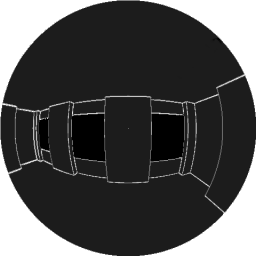
\includegraphics[width=.95\linewidth]{media/radiosity1_eye.png}
	\end{subfigure}
	\begin{subfigure}{0.24\textwidth}
		\centering
		\captionsetup{width=0.95\textwidth, justification=centering}
		\caption*{Patch $\beta$ debajo de $\alpha$,\\ se observa el sol.}
		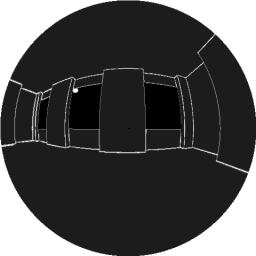
\includegraphics[width=.95\linewidth]{media/radiosity1_eye1.png}
	\end{subfigure}%
	\begin{subfigure}{0.24\textwidth}
		\centering
		\captionsetup{width=0.95\textwidth, justification=centering}
		\caption*{Patches iluminados,\\ durante pasada 1.}
		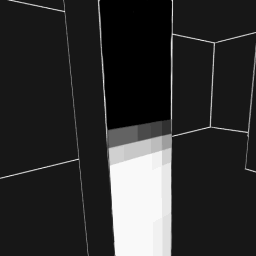
\includegraphics[width=.95\linewidth]{media/radiosity_patch2.png}
	\end{subfigure}%
	\begin{subfigure}{0.24\textwidth}
		\centering
		\captionsetup{width=0.95\textwidth, justification=centering}
		\caption*{Vista desde patch $\alpha$,\\ después de pasada 1.}
		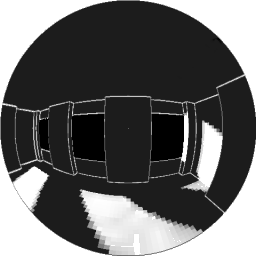
\includegraphics[width=.95\linewidth]{media/radiosity2_eye.png}
	\end{subfigure}
	\label{fig:radiosity1}
\end{figure}%
\begin{figure}[H]
	\centering
	\begin{subfigure}{0.24\textwidth}
		\centering
		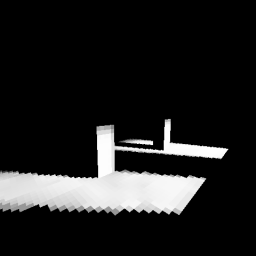
\includegraphics[width=.95\linewidth]{media/radiosity1.png}
		\captionsetup{width=0.95\textwidth, justification=centering}
		\caption*{Pasada 1.}
	\end{subfigure}%
	\begin{subfigure}{0.24\textwidth}
		\centering
		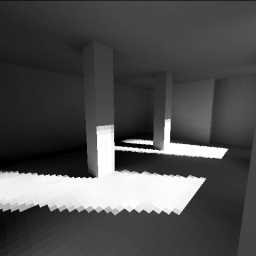
\includegraphics[width=.95\linewidth]{media/radiosity2.png}
		\captionsetup{width=0.95\textwidth, justification=centering}
		\caption*{Pasada 2.}
	\end{subfigure}%
	\begin{subfigure}{0.24\textwidth}
		\centering
		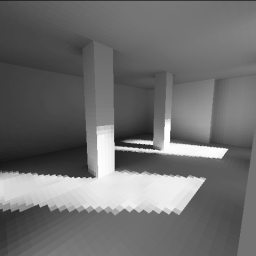
\includegraphics[width=.95\linewidth]{media/radiosity3.png}
		\captionsetup{width=0.95\textwidth, justification=centering}
		\caption*{Pasada 3.}
	\end{subfigure}
	\begin{subfigure}{0.24\textwidth}
		\centering
		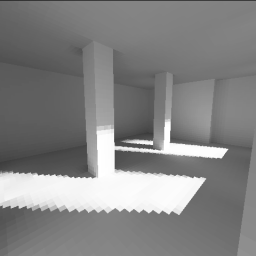
\includegraphics[width=.95\linewidth]{media/radiosity16.png}
		\captionsetup{width=0.95\textwidth, justification=centering}
		\caption*{Pasada 16.}
	\end{subfigure}
	\caption{Ejemplo de varias pasadas de radiosidad sobre una escena \cite{hugo2000}.}
	\label{fig:radiosity2}
\end{figure}


\subsubsection{Radiosidad}
\label{subsec:radiosity}

Radiosidad es una aproximación con elementos finitos para el cómputo del transporte de luz global. Esta técnica fue introducida por Goral y otros en 1984 \cite{goral84}. La idea general es discretizar las superficies de la escena en elementos finitos de éstas, estos elementos son usualmente llamados \emph{patches} (parches o trozos) los cuales son utilizados para calcular el transporte de luz entre ellos como se observa en la figura \ref{fig:radiosity2}. Esto conlleva a ciertas implicaciones; de cada \emph{patch} se necesita guardar el valor de radiosidad para las superficies difusas, o la distribución direccional de la luz saliente y entrante para superficies no difusas.

\subsubsection{Trazado de Rayos e Integración Monte Carlo}
\label{subsec:monte_carlo_raytracing}
La ecuación de renderizado puede ser aproximada utilizando el algoritmo de trazado de rayos o \emph{ray tracing}, esta es una técnica basada en integración Monte Carlo. Para aproximar la propagación de la luz sobre un punto se crea un número considerable de muestras en variadas direcciones, luego por cada muestra se evalúa la ecuación de renderizado y el promedio de todos los resultados converge hacia la solución analítica de la ecuación de renderizado sobre ese punto. Para evaluar una muestra la luz incidente desde una dirección tiene que ser calculada, para esto un rayo de luz es enviado en una dirección y la luz emitida desde el primer punto de colisión es calculada evaluando la ecuación de renderizado en este punto.

Ray tracing está dividido en dos categorías: forward y backward. Forward ray tracing consiste en lanzar las trazas/rayos de luz desde las fuentes de luz y usar aquellos que llegan a la cámara. Backward ray tracing por el contrario lanza las trazas/rayos de luz desde la cámara y traza el camino de estos a través de la escena \cite{Arvo86backwardray}.

\begin{figure}[H]
	\centering
	\begin{subfigure}{0.33\textwidth}
		\centering
		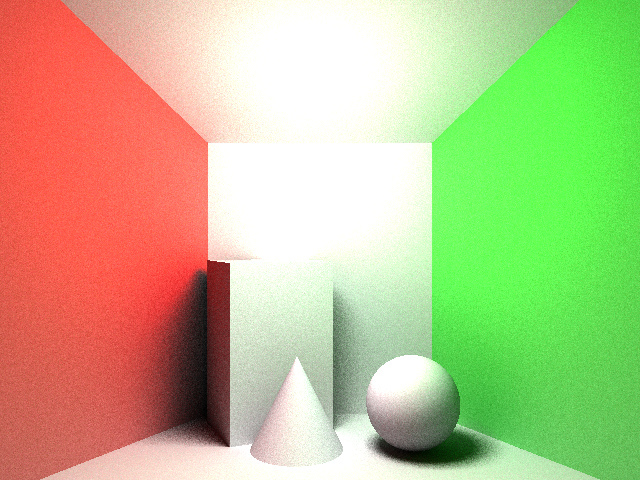
\includegraphics[width=.98\linewidth]{media/ray_100s.jpg}
		\captionsetup{width=0.98\textwidth, justification=centering}
		\caption*{100 muestras rayos/píxel,\\ 50 para luces de área.}
	\end{subfigure}%
	\begin{subfigure}{0.33\textwidth}
		\centering
		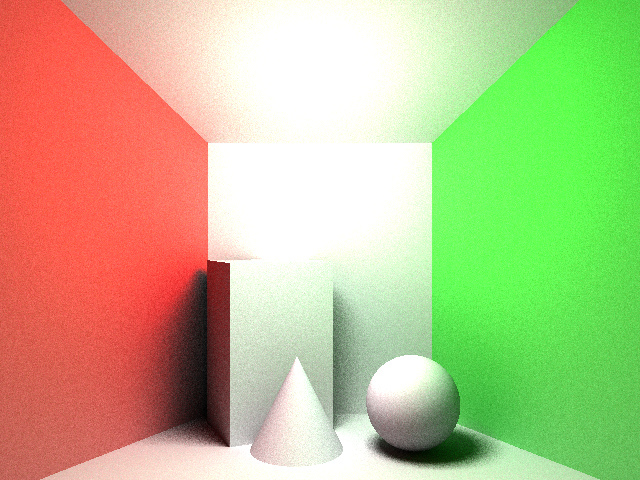
\includegraphics[width=.98\linewidth]{media/ray_500s.jpg}
		\captionsetup{width=0.98\textwidth, justification=centering}
		\caption*{500 muestras rayos/píxel,\\ 50 para luces de área.}
	\end{subfigure}%
	\begin{subfigure}{0.33\textwidth}
		\centering
		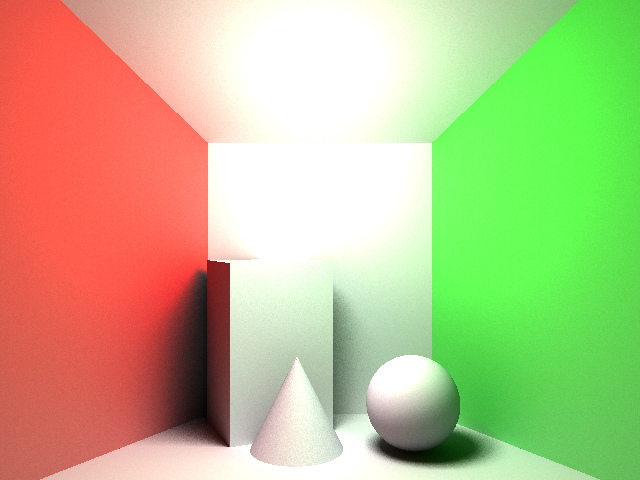
\includegraphics[width=.98\linewidth]{media/ray_1000s.jpg}
		\captionsetup{width=0.98\textwidth, justification=centering}
		\caption*{1000 muestras rayos/píxel,\\ 100 para luces de área.}
	\end{subfigure}
	\caption{Ray tracing sobre una escena, se puede observar mayor calidad y reducción de ruido al aumentar la cantidad de muestras \cite{locdoraytracing}.}
	\label{fig:ray_tracing_nsamples}
\end{figure}